\begin{frame}{}
	\centering \textbf{\huge Bipartite graphs}
\end{frame}

\begin{frame}{Hall's Theorem}
\only<1>{
\begin{figure}
\end{figure}
}
\begin{block}{Definition}
	\only<1>{A bipartite graph $G(U, W, E)$, has a matching satisfying $U$ if and only if $|N(X)| \geq |X|$ for every nonempty subset $X \subseteq U$.}
\end{block} 
\end{frame}

\begin{frame}{Examples - Hall's Theorem}
- Examples on the board --

\end{frame}
  
\begin{frame}{Königs Theorem}
\only<1>{
\begin{figure}
\end{figure}
}
\begin{block}{Definition}
    \only<1>{The maximum matching for a bipartite graph equals its minimum vertex cover}
\end{block} 
\end{frame}

\begin{frame}{Königs Theorem - Example}
-- Example on the Board -- 
  
\end{frame}

\begin{frame}{Alternating Path}
\centering
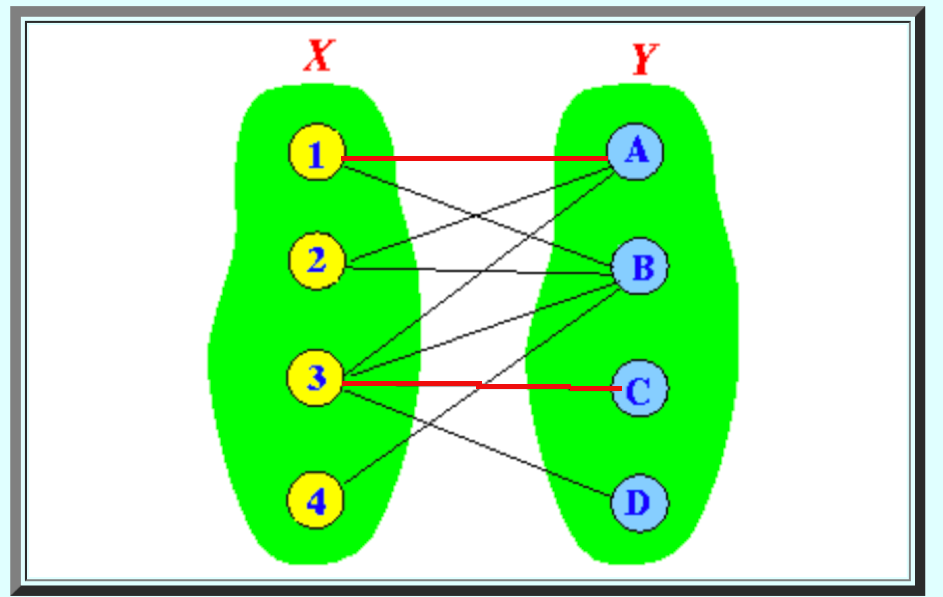
\includegraphics[width=.4\linewidth]{img/bipartite/alternating1.png}
\only<1>{
\begin{figure}
\end{figure}
}
\begin{block}{Definition}
    \only<1>{Let $G = (X, Y, E)$ be a bi-partite graph where the vertices are divided into the sets X and Y and E the edges.}
\end{block} 
\end{frame}

\begin{frame}{Alternating Path}
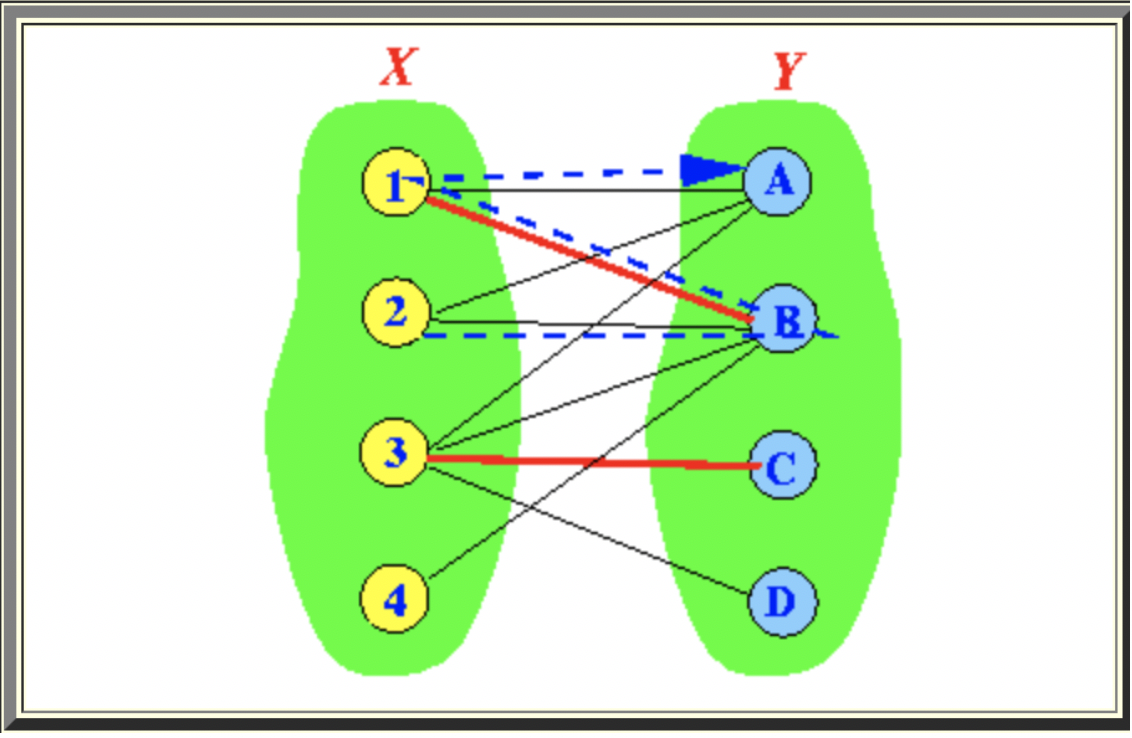
\includegraphics[width=.8
\linewidth]{img/bipartite/alternating2.png}
  
\end{frame}

\begin{frame}{Alternating Path}
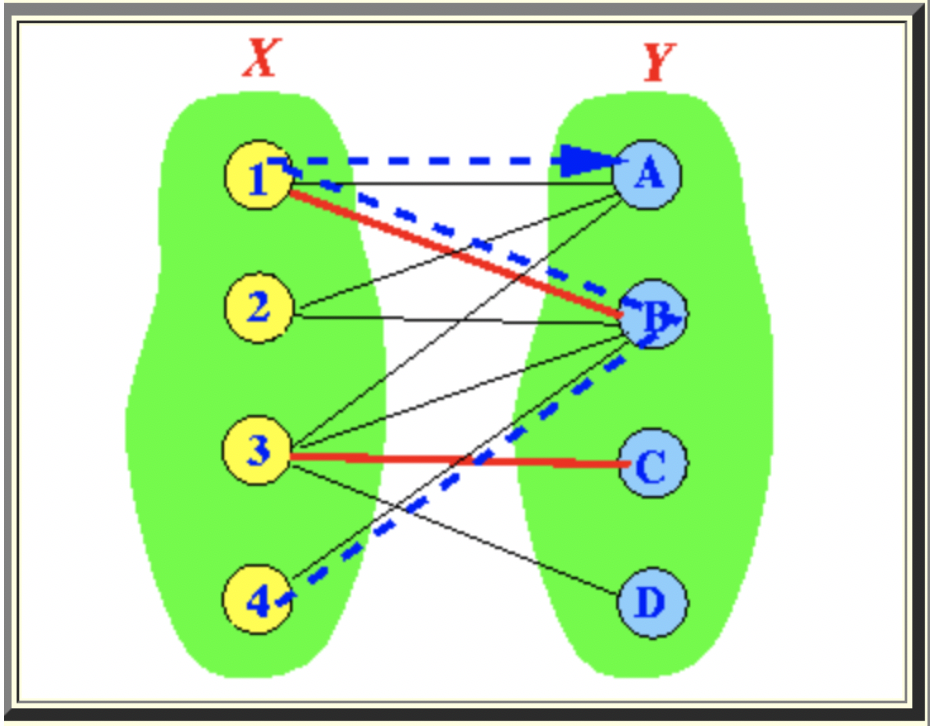
\includegraphics[width=.8\linewidth]{img/bipartite/alternating3.png}
  
\end{frame}

\begin{frame}{Alternating Path - Summary}
- starts in a vertex element of X and ends in vertex element of Y\newline
- must have an odd-number of edges\newline
- will visit nodes in X und Y alternatedly\newline
- And it starts and ends in free/unmatched vertices\newline
\newline
$\rightarrow$ To go forward, use an edge that is not part of the matching\newline
$\rightarrow$ To go backward, use an edge that is part of the matching\newline
  
\end{frame}

\begin{frame}{Augmenting Path - Definition}
\only<1>{
\begin{figure}
\end{figure}
}
\begin{block}{Definition}
    \only<1>{An augmenting path is an alternating path where the first and last vertex are unmatched.}
\end{block} 
\end{frame}

\begin{frame}{Augmenting Path - example}
-- Example on the Board --
  
\end{frame}

\begin{frame}{Breadth First Search - repetition}
-- Example on the Board --
  
\end{frame}

\begin{frame}{Berge Theorem}
A matching is a maximum matching if it contains no augmenting path.
  
\end{frame}

\begin{frame}{Hungarian Method}
Search augmenting paths in the graph until no augmenting path can be found\newline
\newline
$\rightarrow$ \textbf {Time complexity: $O(|V|^3)$}\newline
\newline
Precise information can be found here: \textbf {https://brilliant.org/wiki/hungarian-matching/}\newline
\newline
\textbf {Note}: It is not an algorithm, so it does not specify a implementation
\end{frame}

\begin{frame}{Maximum Flow Reduction}
-- Example on the Board --
  
\end{frame}

\begin{frame}{Hopcraft-Carp Algorithm}
Input: \textbf{A bipartite Graph}
Initialize Matching\newline
1. Repeat\newline
$\rightarrow$ Build alternating level graph rooted at unmatched vertices using bfs\newline
$\rightarrow$ Augment M via maximal set of vertex disjoint shortest-length paths\newline
$\rightarrow$ until no augmenting paths exists\newline
2. Return M\newline
		
\textbf {Time complexity: $O(|E|*\sqrt{|V|})$}
  
\end{frame}

\begin{frame}{Hopcraft-Carp Algorithm - bipartite Graph}

-- Example on the Board --
  
\end{frame}
